\section{COMPONENT CODE GENERATOR}

\subsection{Source Code Structure}
The generator is packaged in a JAR Java file, under the reverse domain name
cl.alma.acs.ccg which follow the Java package folder structure.

\begin{verbatim}
cl.alma.acs.ccg/
|-- cl/
|   `-- alma/
|       `-- acs/
|           `-- ccg/
|               `-- mwe/
|               |   |-- CppWorkflow.mwe
|               |   |-- JavaWorkflow.mwe
|               |   |-- PythonWorkflow.mwe
|             |   
|               |-- strategy/
|               |   |-- CodeCppGeneration.java
|               |   |-- CodeJavaGeneration.java
|               |   |-- CodePythonGeneration.java
|               |   |-- ContextCodeGeneration.java
|               |   |-- ICodeGenerationStrategy.java
|             |   
|               `-- vetostrategy/
|               |   `-- ACSCCGVetoStrategy.java
|             |     
|               |-- vo/
|                   `-- VOGenerator.java
|
`── templates/
    `-- java/
        |-- AllOverride.xpt
        |-- CDB.xpt
        |-- CommonRoot.xpt
        |-- IDLCommon.xpt
        |-- IDLComp.xpt
        |-- Implements.xpt
        |-- info.xpt
        |-- Interfaces.xpt
        |-- JAVAChComp.xpt
        |-- JAVAComp.xpt
        |-- JAVAHelper.xpt
        |-- JavaRoot.xpt
        |-- Makefile.xpt
        |-- Override.xpt
        |-- SchemaRoot.xpt
        |-- Schema.xpt
        `-- util.ext
\end{verbatim}

\subsubsection{Class Diagram}
In the class diagram, the only classes not developed (in the project) are those
which belongs to the packages {\tt org.eclipse.xpand2.output}  and {\tt
org.eclipse.emf.mew.core}.\\ 
\begin{figure*}[h!t]
\begin{center}
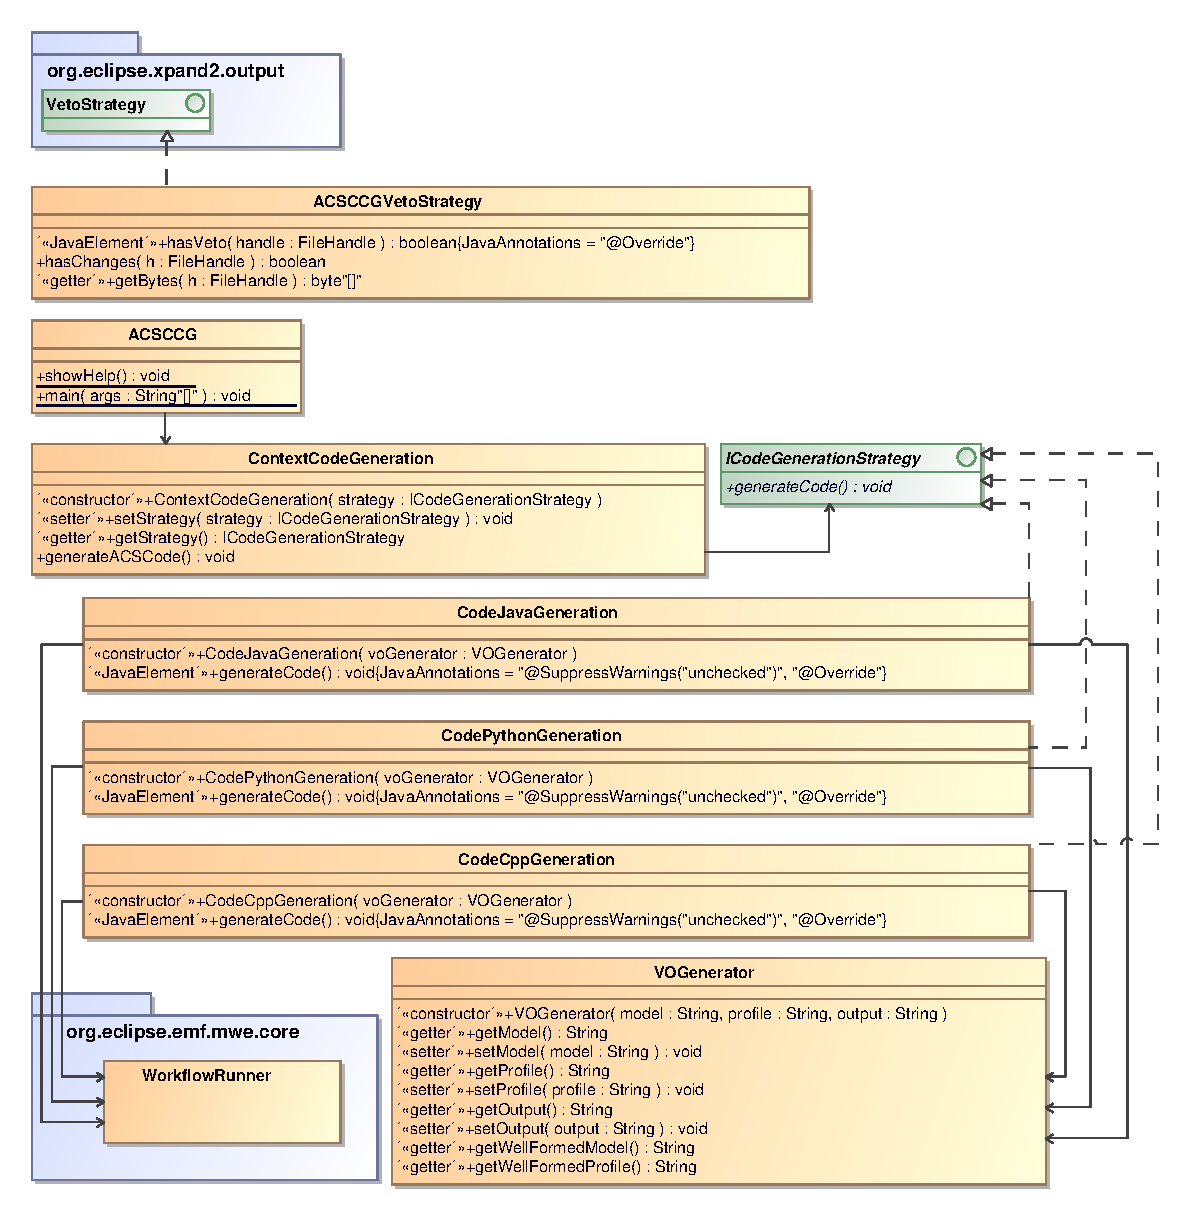
\includegraphics[scale=0.85]{images/ccgclassdiagram}
\caption{\label{fig:main_diag}Component Code Generator Class Diagram}
\end{center}
\end{figure*}

\newpage

\subsubsubsection{Strategy Pattern}
A Strategy Pattern (Policy Pattern) was implemented in the component code
generator to generate the code for each programming languaje in ACS whithout
change top levels algorithms, due to the scope of the project, only Java
strategy is full implemented. 
\begin{figure*}[h!t]
\begin{center}
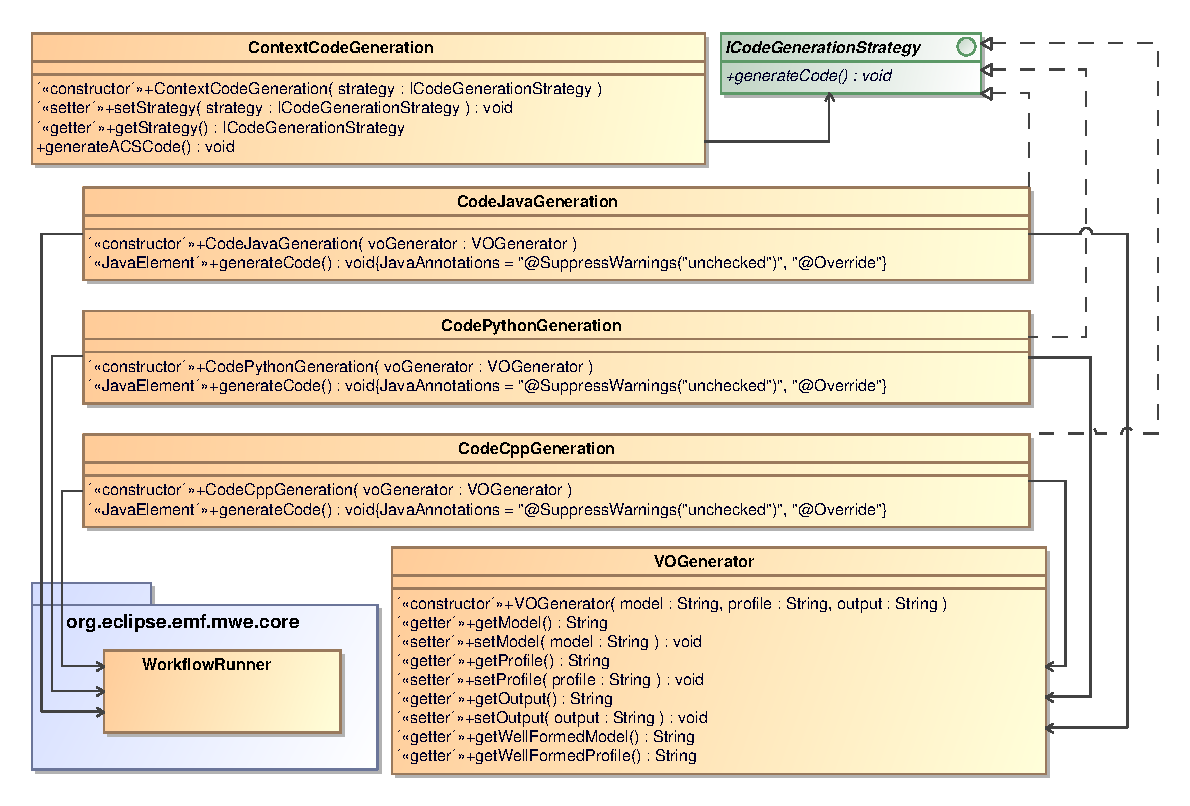
\includegraphics[scale=0.85]{images/strategypattern}
\caption{\label{fig:sp_diag}Strategy Pattern}
\end{center}
\end{figure*}
\\The {\tt ContextCodeGeneration} is the main class to be called for implement
the generator in plugins, Java programs or other enviroments.

\newpage

\subsubsubsection{EMF Veto Strategy}
The class {\tt ACSCCGVetoStrategy} is called by WorkflowRunner in runtime of
the component code generator, for more info about Veto, see Generator
Optimization section in this document. 
\begin{figure*}[h!t]
\begin{center}
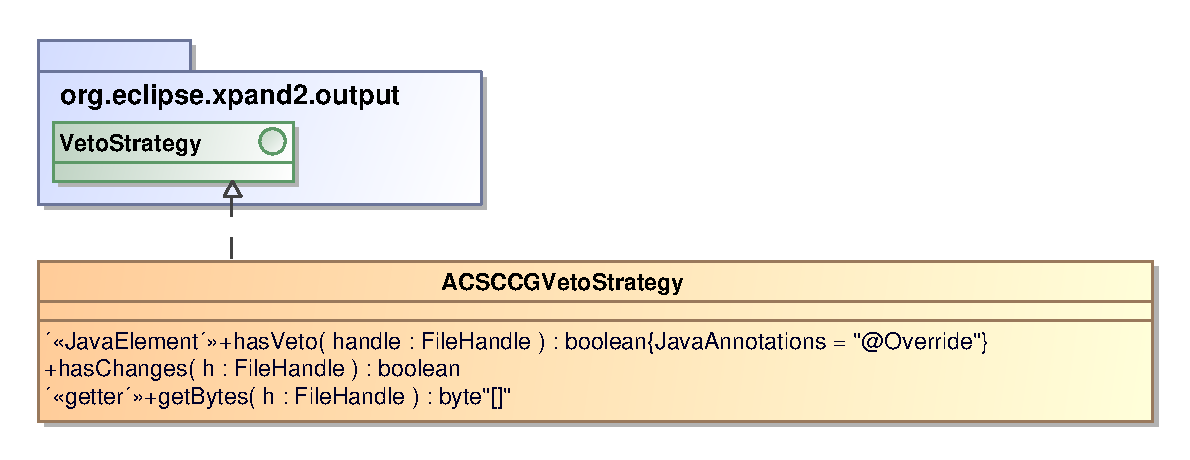
\includegraphics[scale=0.65]{images/vetostrategy}
\caption{\label{fig:vs_diag}EMF Veto Strategy}
\end{center}
\end{figure*}

\newpage

\subsubsection{Sequence Diagram}
To be implemented
\subsubsection{Process Diagram}
To be implemented

\subsection{Stand-alone Generator}
The component code generator was designed to be a stand-alone code generator,
this means, can be executed in any O.S. as a Java Program, JAR Package or
Eclipse Plugin. More info how to use, see the Quick How To section in this
document.\\
\\
The generator supports three ways to be a standa-lone :
\begin{itemize}
  \item JAR Package : The binary files are packaged in a JAR Java file.
  \item Eclipse Plugin : A simple Eclipse plugin.
  \item Command Line : A Java command line program.
\end{itemize}
Also, the generator contains all the packages to be executed without EMF and 
can be imported to other environments running Java.

%-----------begin.gzamora-------------------------------------------------------------------------
\subsection{Notification Channel}

The ACS Notification Channels API provides all the necessary to allow the
communication of data between components. In more detail, this is the minimal
list of a necessary set of components.

\begin{itemize}

\item Channel Data:\\\\ This struct provides the sharing of data events between
two or more diffent components. Basically consists in common data types:
 	 \begin{itemize}
 	 	\item A common data
 	 	\item A common Channel name
 	 \end{itemize}

\item Simple Supplier:\\\\ This component has the function of control over all
the data in the context of send the events to the Notification Channel:
 	 \begin{itemize}
 	 	\item Send simple data events
 	 	\item Send special data events
 	 	\item Data control in case of problems
 	 \end{itemize}
\item Consumer:\\\\ This component has the functionality of obtain all the data
from the common Notification Channel. The consumer gets the data automatically
when a event is available on the Notification Channel.
 	 \begin{itemize}
 	 	\item Receive the data events
      \end{itemize}      

\item Simple Supplier Client:\\\\ This client activate the Simple Supplier
component and set the user data events to send between the Simple Supplier and
the Consumer.

\item Consumer Client:\\\\ This client maintains the activation of the Consumer
component to receive the data events from the Notification Channel

\end{itemize}

\subsubsection{Diagrams}

This is a overview of the Notification Channel implementation on the ACS Code Generator

\begin{figure*}[h!t]
\begin{center}
\includegraphics*[scale=0.75]{images/notificationchannel}
\caption{\label{fig:not_chan}Example Notification Channels class diagram}
\end{center}
\end{figure*}

%
%\begin{figure*}[h!t]
%\begin{center}
%\includegraphics*[scale=0.4]{images/NC}
%\caption{\label{fig:main_diag}Notification Channels dependency diagram}
%\end{center}
%\end{figure*}
%
%\newpage
%\begin{figure*}[h!t]
%\begin{center}
%\includegraphics*[scale=0.8]{images/NC3}
%\caption{\label{fig:main_diag}Notification Channels Supplier secuence diagram}
%\end{center}
%\end{figure*}

%\begin{figure*}[h!t]
%\begin{center}
%\includegraphics*[scale=0.8]{images/NC4}
%\caption{\label{fig:main_diag}Notification Channels Consumer secuence diagram}
%\end{center}
%\end{figure*}

The generator provides a fully implementation of all the necessary to make use
of this functionality. The code is generated in base of the Notification
Channel UML Model, taken attributes and operations from the model and building
a customizable Supplier-Consumer structure. The code generated in detail:
\begin{verbatim}
src-gen/
|-- config/
|   `-- CDB/
|       `-- MACI/
|           |-- Channels/
|           |   `-- mychanneldata
|           |       `-- mychanneldata.xml
|           |-- Components/
|           |   `-- Components.xml
|           `-- Managers/
|               `-- Manager/
|                   `-- Manager.xml
|-- idl/
|   |-- MyConsumerBase.idl
|   |-- MyConsumerClientBase.idl
|   |-- MySimpleSupplierBase.idl
|   |-- MySimpleSupplierClientBase.idl
|   `-- NCCommon.idl
`-- src/
    |-- Makefile
    `-- alma/
        `-- acsgenerator/
            `-- NC/
                |-- MyConsumerBase.java
                |-- MyConsumerBaseHelper.java
                |-- MyConsumerClientBase.java
                |-- MySimpleSupplierBase.java
                |-- MySimpleSupplierBaseHelper.java
                `-- MySimpleSupplierClientBase.java
\end{verbatim}

In the tree view is possible see three sub directories:
\begin{itemize}
 	 \item config: Includes the manager, components and notification channel configurations to the CDB.
 	 \item idl: Includes the IDL Interfaces for the Supplier, Consumer, clients and the common data to share.
 	 \item src: Includes the source code of the Supplier and Consumer components and clients.
\end{itemize}

%----------end.gzamora---------------------------------------------------------------

\subsection{Inheritance}

\subsubsection{Multiple Level}
The generator can support inheritance in one ore more inherited levels
with the ability to override the inherited methods from the parenet, or,
override all methods inherited in all inherited levels.\\
This can be viewed in figure 5.

\begin{figure*}[h!t]
\begin{center}
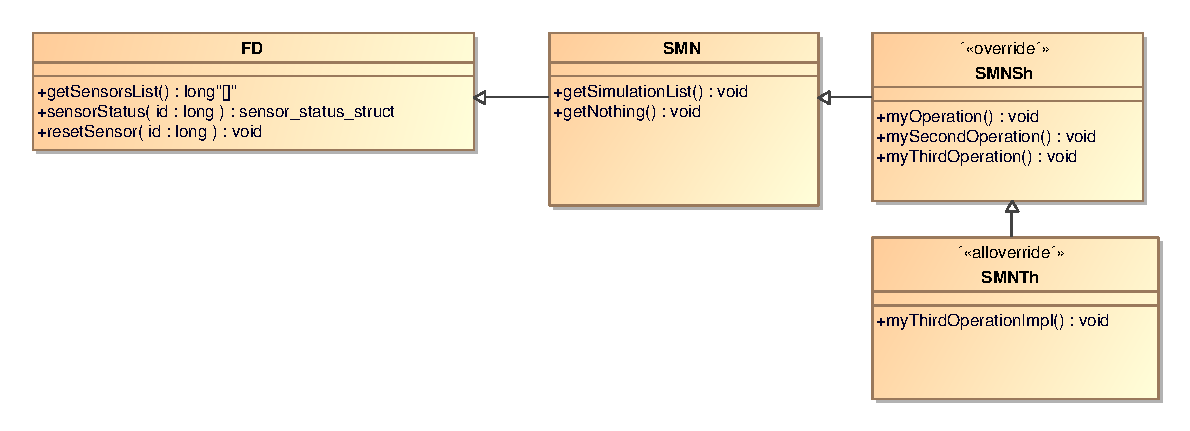
\includegraphics[scale=0.75]{images/simpleinheritance}
\caption{\label{fig:vs_diag}Inheritance in the generator}
\end{center}
\end{figure*}

The class SMN is extended from FD class and inherits implicitly the methods
from FD without override them.\\ 
The class SMNSh is extended from SMN, and override the methods from SMN.\\
The class SMNTh is extended from SMNSh and override all methods inherited, the
methos from FD, SMN and SMNh.\\
\\
A stereotype will differentiate if the class generated must apply the override
policy in the inhertance.

\subsubsubsection{Characteristic Component}
A class with the stereotype \verb+<<Characteristic>>+, if is extended from
other class, the generator will not implement the inheritance in the Java code,
because the Java OOP paradigm not support multiple inheritance (parallel
inheritance) and the class with \verb+<<Characteristic>>+, the generator will
generate the class already extended from ACS class 'CharacteristicComponentImpl'.
 
\subsubsection{Interface}
The inheritance can be applied to Interface Classes, the interface will not
override the methods (Java OOP aspect) from the super-interface (parent
interface). But, the class will have to implement the methods from child
Interface and all his inherited methods.\\
\begin{figure*}[h!t]
\begin{center}
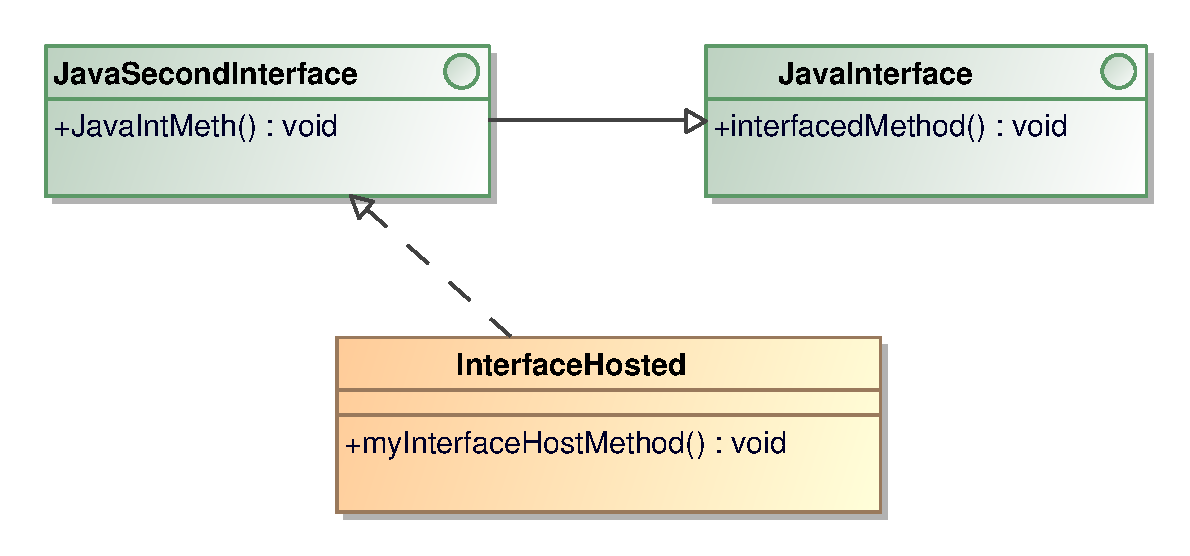
\includegraphics[scale=0.45]{images/interfaceinheritance}
\caption{\label{fig:vs_diag}Inheritance in interfaces.}
\end{center}
\end{figure*}

\newpage

\subsection{Interfaces and Abstract classes}
For desing pattern implementations, the generator support basic features of
Java OOP as Interfaces or Abstract Classes.
\subsubsection{Interface Classes}
The generator support the interface implementation specified in the model and
provides the generated code under the Java OOP standard. It follow the OOP Java
Paradigm.\\
Any class can implemented one or more interfaces, the methods implemented from
the interface will be generated.
An example of this can be viewed in Figure 8.
\begin{figure*}[h!t]
\begin{center}
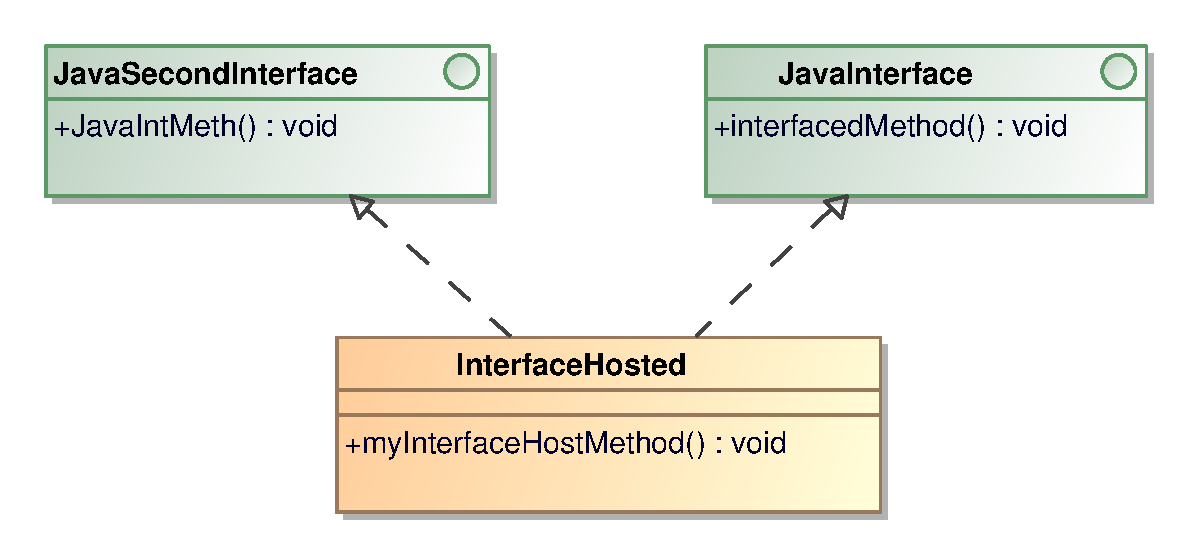
\includegraphics[scale=0.6]{images/interface}
\caption{\label{fig:vs_diag}Interface Example}
\end{center}
\end{figure*}

Will generate :
\begin{verbatim}
public class InterfaceHosted implements ComponentLifecycle,
InterfaceHostedOperations, JavaInterface, JavaSecondInterface {
...
}
\end{verbatim}

\subsubsection{Abstract Classes}
Same as interface implementation, the generator support the abstract class
definition and generate the code.\\
Classes with the \verb+<<Characteristic>>+ stereotype, the generator will no
generate this classes as Abstract.

\subsection{Implemented Code v/s Generated Code}
In every model driven development and code generators, is important how make a
strategy to separate the code already generated with the code implemented over
the generated code.\\
They are three ways solve this.

\subsubsection{EMF Veto Strategy and Inheritance}
The Veto EMF strategy (see Generator Optimization section) is a good solution
using inheritance to implement new things, but, must be create a new class for every change in our code to void
override the whole code already generated, so, this is not the best solution,
but, it works.

\subsubsection{GAP Desing Pattern}
The generation GAP desing pattern provides separate the code with all
hand-modifications implemented in sub-classes, this mean that the core classes
are generated only once and the hand-made implementations, are extended as
subclases from core classes.

\subsubsection{Protected Areas}
Xpand, provides protected areas to our generated code, this mean, that certain
areas with the protected tag with a unique autegenerated ID, can be modified by
the developer without loosing the hand-modifications over the generated code
when the code is re-generated (even if classes are changed in the model).
i.e.: This code went generated with protected areas.
\begin{verbatim}
1. public void getSimulationList() {
2. /*PROTECTED REGION ID(getSimulationList) ENABLED START*/
3.    //Implementation Method here!
4. /*PROTECTED REGION END*/
5. }

1. Method definition
2. Start Protected Area
3. Method hand implementation
4. End Protected Area
\end{verbatim}
Protected areas are specified in generator templates, the generator analize the
generated code, check the code with the template, and protect the area from the
regeneration. If the protected region is not in the templates, the generator
will void the area.\\
In methods, only the implementation is protected and for the code that scape
from UML model every class has a protected area for custom imports, variables and methods.
